\chapter{Resultados e Discussões}
\label{cap:resultados}

Neste capítulo, apresentamos os resultados obtidos a partir das experimentações práticas do Escalonador Adaptativo de Compactações implementado no RocksDB. O objetivo desta avaliação é quantificar os ganhos e \textit{trade-offs} introduzidos pela adaptação dinâmica frente ao agendador estático padrão da literatura (aqui denotado como \textit{Base}). 

A fim de garantir solidez e validade estatística das métricas, todos os cenários de teste foram processados por uma suíte de automação em Python que utiliza a ferramenta interna de benchmark do RocksDB chamada \textit{db\_bench}, a qual executou 25 repetições para cada configuração experimental e computou médias e desvios-padrão. Antes da coleta de dados de cada rodada, o banco de dados foi submetido a 100.000 operações de \textit{warmup} para garantir o pré-aquecimento de \textit{caches} da CPU e do Sistema Operacional.

\section{Metodologia e Definição das Cargas de Trabalho (\textit{Workloads})}

Para avaliar o comportamento da LSM-Tree sob diferentes espectros de estresse, a suíte de \textit{benchmarks} foi segmentada em cinco cargas de trabalho distintas, refletindo padrões de acesso comuns em bancos de dados reais e isolando as variáveis de observação:

\begin{itemize}
    \item \textbf{Carga Mista (\textit{Mixed Workload}):} Utiliza a operação \texttt{readrandomwriterandom} com 1.000.000 de operações e 8 \textit{threads}. O objetivo é simular um cenário de produção comum, onde o banco de dados lida com concorrência severa entre requisições de leitura de usuários e gravações de sistema, avaliando o balanceamento geral.
    \item \textbf{Carga de Pico (\textit{Burst}):} Emprega a operação \texttt{overwrite} processando 800.000 registros e saturando o sistema com 16 \textit{threads}. Esta carga testa a resiliência do sistema sob intenso volume de sobreposição de chaves, avaliando a capacidade do banco de não colapsar frente a picos repentinos de atualização.
    \item \textbf{Escalabilidade (\textit{Scaling}):} Consiste em rodadas incrementais de paralelismo (1, 2, 4, 8 e 16 \textit{threads}) utilizando \texttt{fillrandom}. O objetivo é verificar gargalos de contenção de travas (\textit{lock contention}) à medida que a simultaneidade aumenta.
    \item \textbf{Latência Pura (\textit{Latency}):} Emprega 8 \textit{threads} e injeta valores maiores em tamanho (\textit{value size} de 2000 bytes) com 500.000 operações. É projetada exclusivamente para exacerbar e medir o impacto dos engasgos de compactação (\textit{stalls}) na latência de cauda perceptível aos clientes.
    \item \textbf{Amplificação de Escrita (\textit{WAF}):} Focada na durabilidade do dispositivo, testa o banco com o agendador estático (\textit{baseline}) em contraste com o adaptativo utilizando diversos graus de sensibilidade ($\alpha$). 
\end{itemize}

\section{Ambiente de Avaliação e Metodologia}\label{sec:ambiente}
Os ensaios foram conduzidos em um servidor de alto desempenho, equipado com processador Intel\textsuperscript{\textregistered} Xeon\textsuperscript{\textregistered} Gold 5317 operando a 3.00 GHz, 256 GB de memória RAM convencional e duas unidades de Memória Persistente (PMEM) Intel Optane de 500 GB cada. 

Considerando que as estruturas Log-Structured Merge-Trees sobre armazenamento NVM/PMEM exibem características de desempenho altamente sensíveis ao barramento de memória, as métricas avaliadas compreendem a vazão geral (Throughput, medido em operações por segundo), a penalidade sobre os usuários (Latência de cauda P99) e a durabilidade física do dispositivo subjacente através do Fator de Amplificação de Escrita (WAF). 

\section{Análise do Viés de Escalonamento e Afinidade de CPU}
Um aspecto arquitetural profundo na avaliação de bancos de dados modernos em PMEM é a interferência do escalonador do Sistema Operacional na alocação de \textit{threads}. Como apontado durante a formulação deste projeto, questionou-se se a fixação prévia de processos a determinados núcleos (\textit{CPU pinning}) poderia introduzir um viés nos resultados. Para mitigar esta dúvida, a suíte de \textit{benchmarks} foi executada integralmente em duas instâncias isoladas: \textit{Pinned} (confinando o processo aos núcleos físicos de 0 a 11 via ferramenta \textit{taskset}) e \textit{Unpinned} (delegando total liberdade ao escalonador do \textit{kernel} do Linux).

A análise direta do gráfico \ref{fig:bias_comparison_throughput} e da tabela \ref{tab:bias_throughput} comprova a premissa de sensibilidade da arquitetura. Em cargas altamente concorrentes e mistas, o ambiente livre (\textit{Unpinned}) restringe a vazão em torno de 526 mil operações por segundo. Quando forçamos a afinidade com a CPU, garantindo que o acesso à memória ocorra localmente ao nó NUMA da Intel Optane, o rendimento atinge a marca de $\sim$663 mil operações por segundo (aumento superior a 25\%).  

Este ganho superior a 25\% ocorre porque a PMEM atua como um dispositivo dependente de topologia \textit{Non-Uniform Memory Access} (NUMA). No cenário \textit{Unpinned}, a constante migração de contexto do SO expõe o RocksDB a ciclos excessivos de comunicação inter-soquetes. O viés de \textit{pinning}, portanto, não invalida o ensaio; muito pelo contrário, ele representa o cenário ótimo indispensável para sistemas de bancos de dados orientados a desempenho que desejam extrair o real limite das memórias endereçáveis por \textit{byte}. O restante desta discussão terá como foco primordial os resultados \textit{Pinned}, dada a sua representatividade para configurações corporativas de produção.

\begin{figure}[h]
\centering
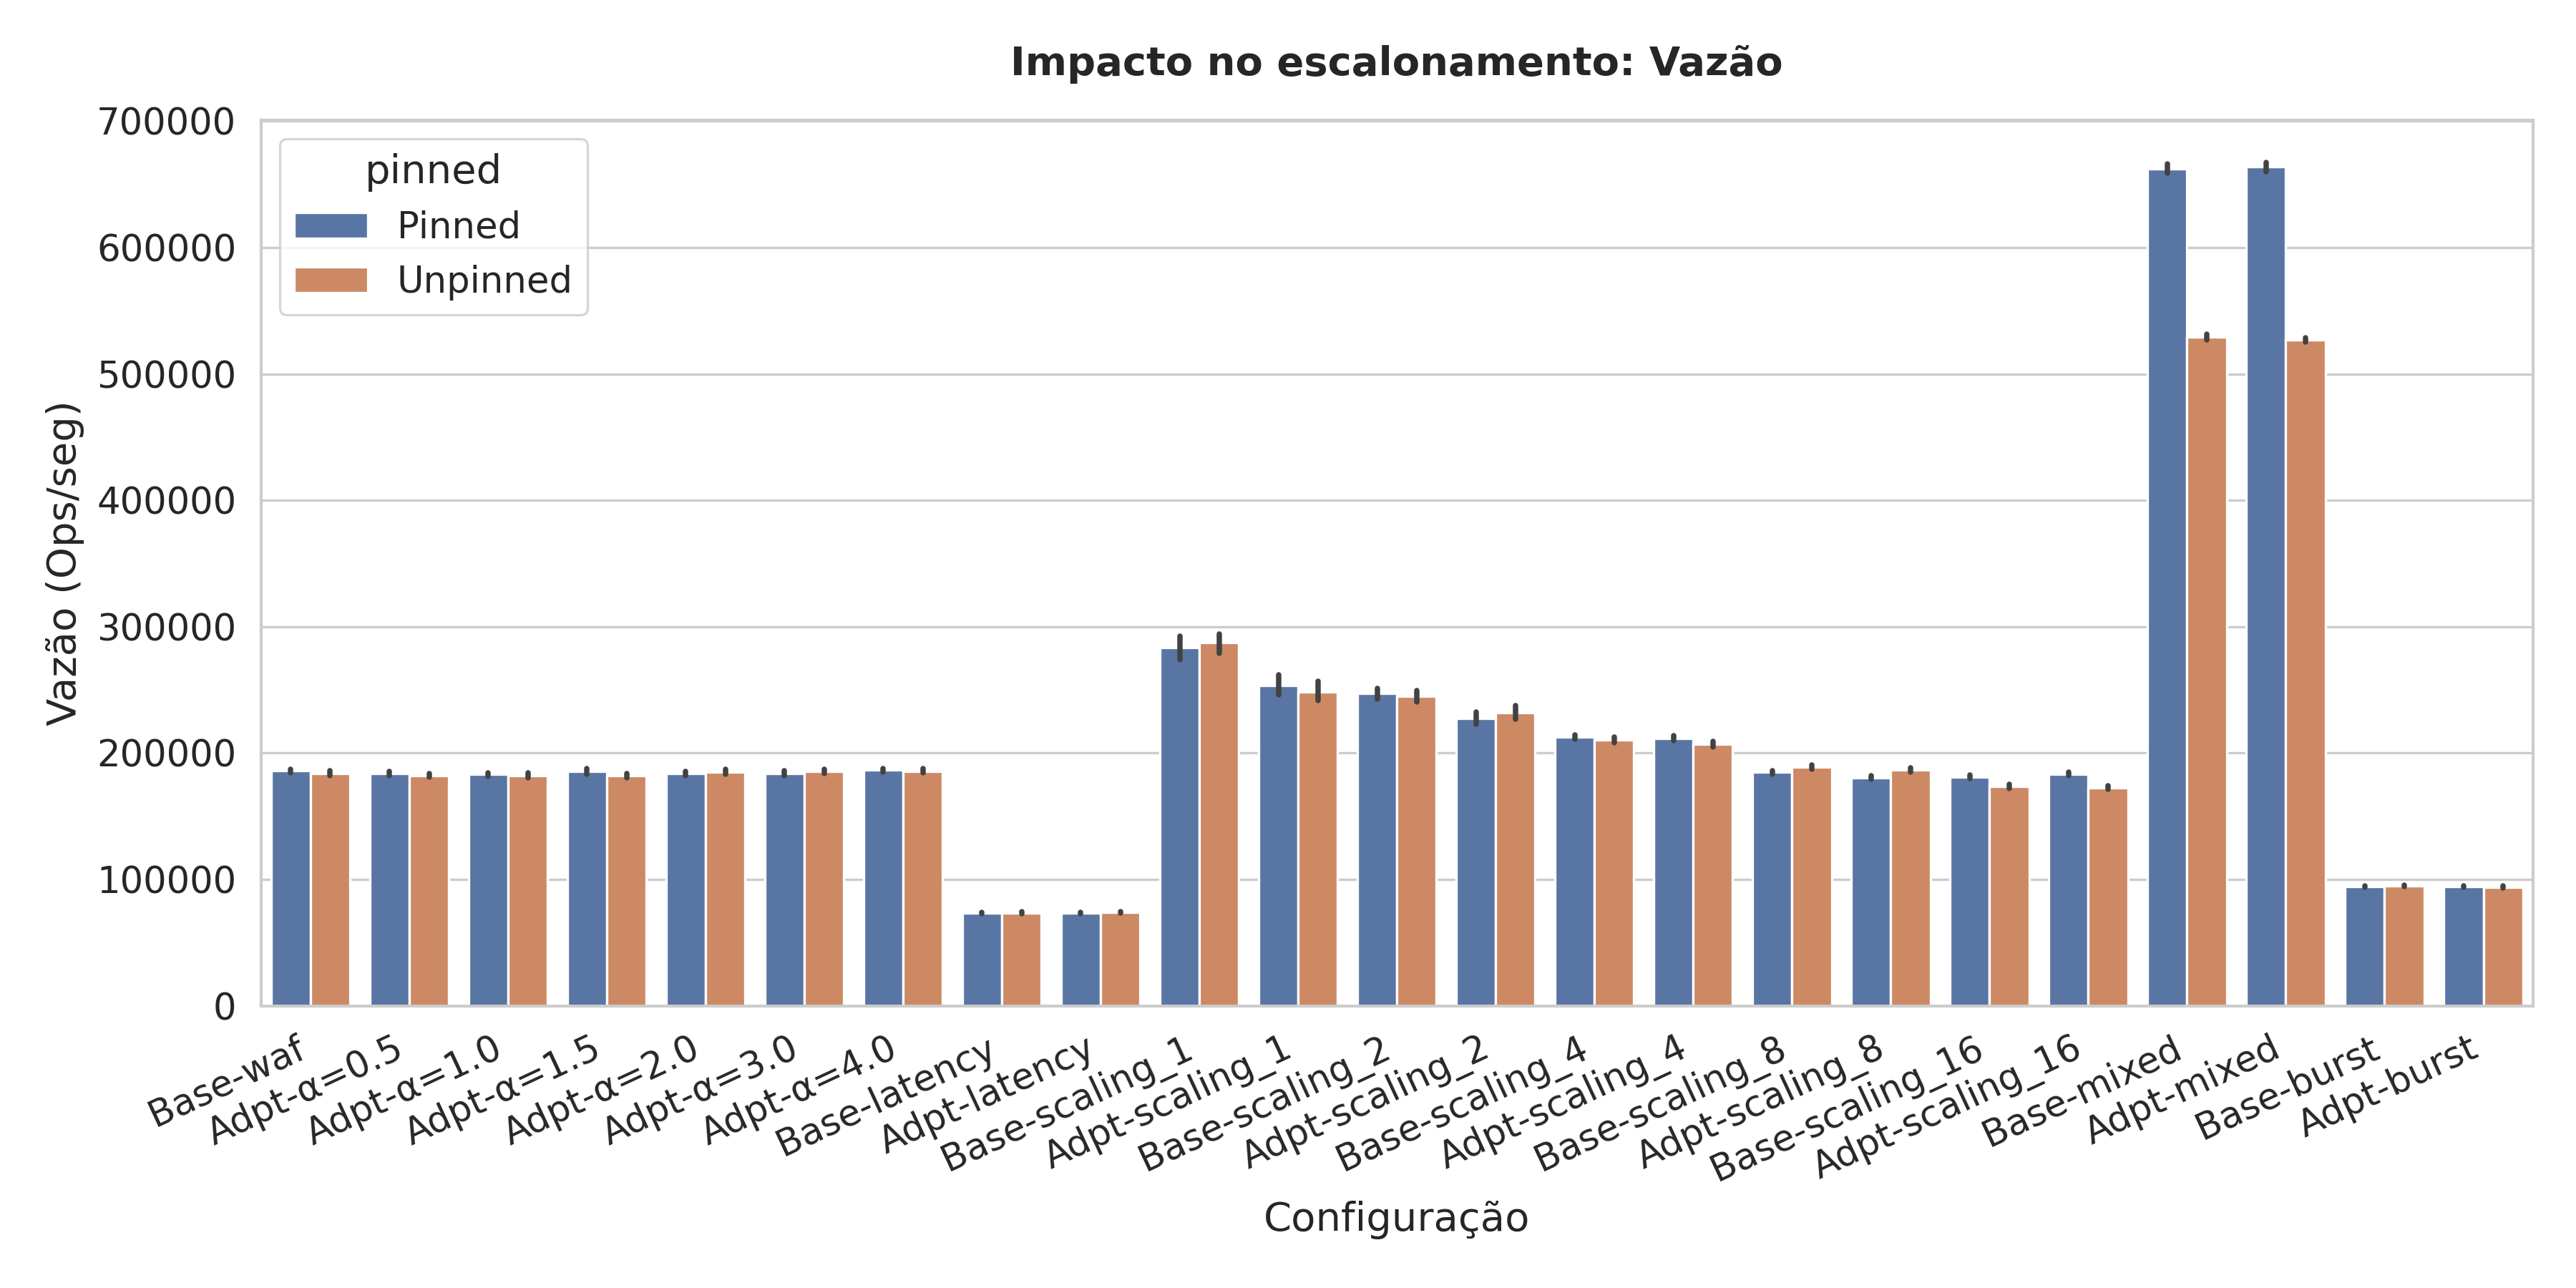
\includegraphics[scale=0.5]{figs/graphs/bias/bias_comparison_throughput.png}
\caption{Comparação direta de ambientes com e sem fixação de recursos. Destaca o viés e a variância do agendador.}
\label{fig:bias_comparison_throughput}
\end{figure}

\begin{table}[h]
\centering
\caption{Comparativo de Vazão Média (ops/sec) com Intervalo de Confiança (95\%)}
\label{tab:throughput_mixed_burst}
\resizebox{\textwidth}{!}{
\begin{tabular}{l|cc|cc}
\hline
\textbf{Configuração} & \textbf{Média Unpinned} & \textbf{IC 95\% Unpinned} & \textbf{Média Pinned} & \textbf{IC 95\% Pinned} \\ \hline
Adpt-mixed & 526.996,0 & \pm 2.055,90 & 663.940,0 & \pm 3.450,21 \\
Base-mixed & 529.296,0 & \pm 2.260,96 & 662.434,0 & \pm 3.587,16 \\
Adpt-burst & 94.072,6  & \pm 612,85   & 94.312,6  & \pm 532,49   \\
Base-burst & 94.720,8  & \pm 598,13   & 94.468,5  & \pm 486,40   \\ \hline
\end{tabular}
}
\end{table}

\section{Comportamento da Vazão Sistêmica (Throughput)}
O gráfico \ref{fig:throughput_pinned} (\textit{Pinned Environment}) com os dados que estão descritos na Tabela \ref{tab:throughput_pinned} evidencia o desempenho bruto dos mecanismos sob diferentes variações paramétricas do agendador e do grau de paralelismo. Uma métrica primordial de aceitação de qualquer componente adaptativo reside na confirmação de que sua \enquote{Função de Utilidade}, responsável por calcular o peso dinâmico de PMem e de CPU, não gere \textit{overhead} destrutivo.

\begin{figure}[h]
\centering
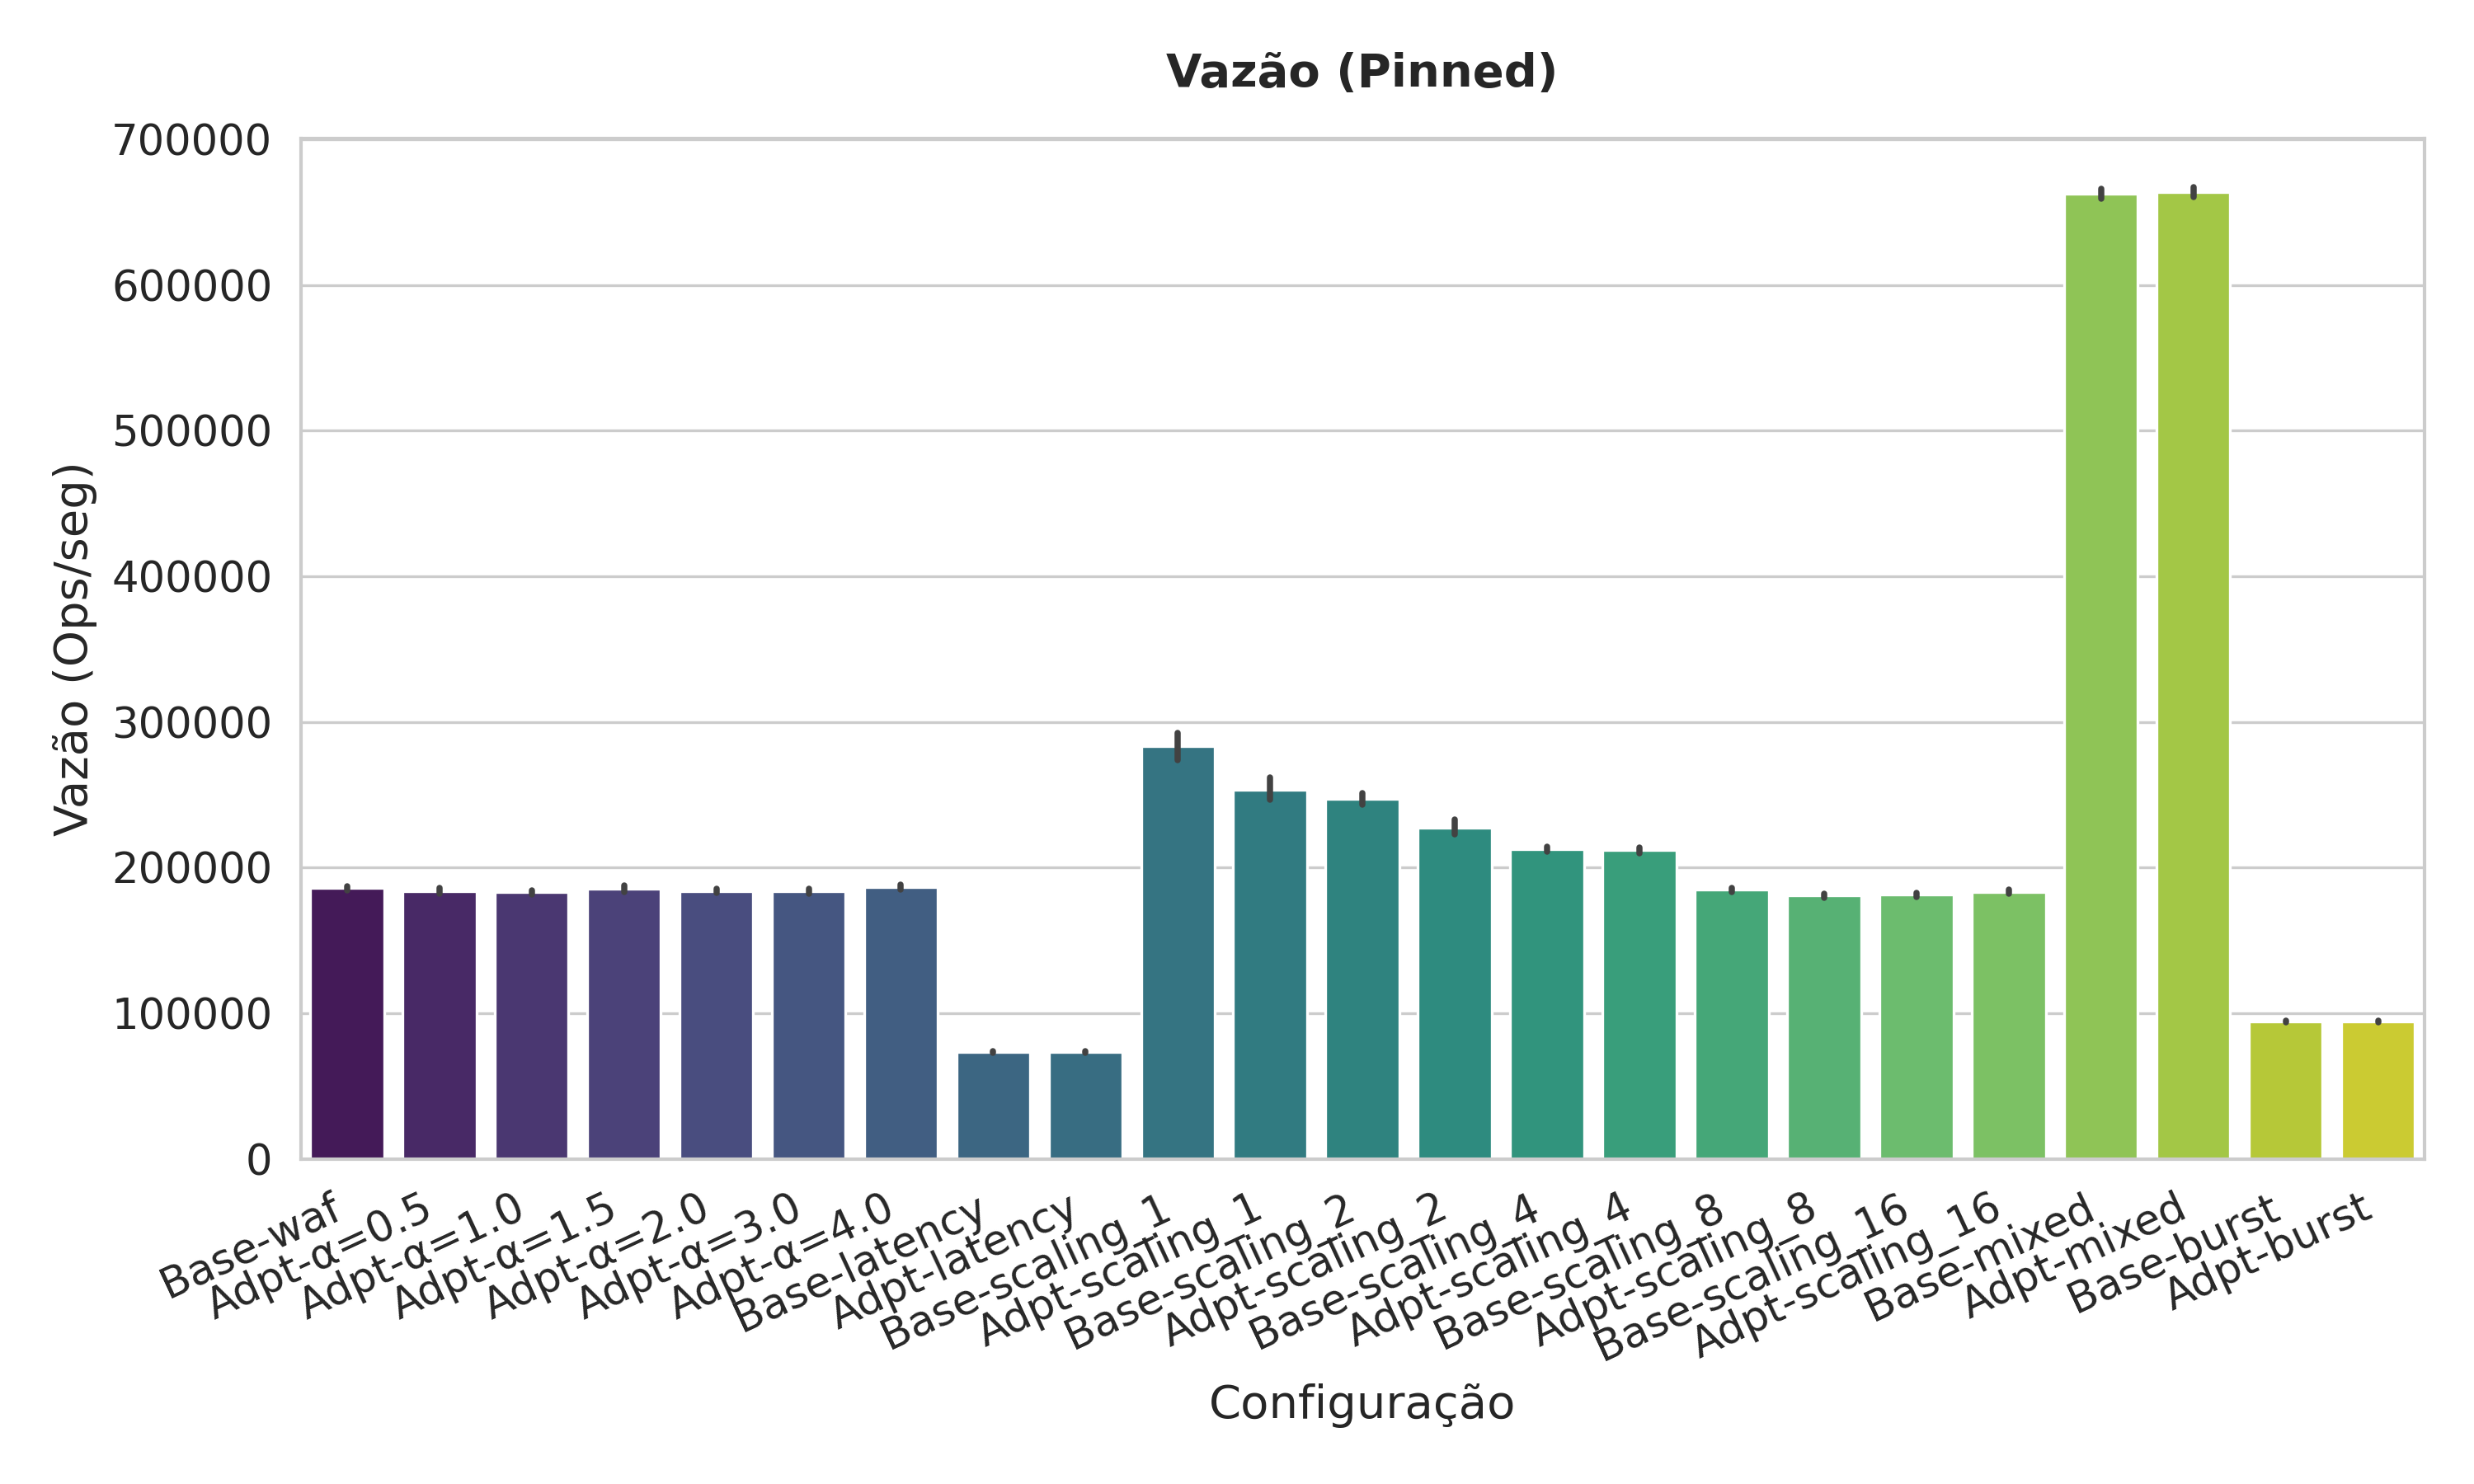
\includegraphics[scale=0.5]{figs/graphs/pinned/throughput.png}
\caption{Vazão geral (operações por segundo) em todas as configurações. Quanto maior, melhor.}
\label{fig:throughput_pinned}
\end{figure}

\begin{table}[h]
\centering
\caption{Resumo Estatístico de Throughput (Operações/seg) - Ambiente Pinned}
\label{tab:throughput_pinned}
\begin{tabular}{lcc}
\hline
\textbf{Configuração} & \textbf{Média (ops/sec)} & \textbf{Desvio Padrão} \\ \hline
Base-mixed & 662.433 & 9.319 \\
Adpt-mixed & 663.940 & 9.174 \\
Base-burst & 94.468 & 1.266 \\
Adpt-burst & 94.312 & 1.430 \\
Base-scaling\_16 & 181.293 & 3.428 \\
Adpt-scaling\_16 & 183.445 & 3.396 \\ \hline
\end{tabular}
\end{table}

Observamos que o algoritmo Adaptativo opera estatisticamente em paridade com o modelo Base do RocksDB, apresentando sutil superioridade técnica no cenário de uso misto e no máximo nível de paralelismo (\textit{scaling\_16}). Tais evidências indicam que a Função de Utilidade de CPU/PMEM possui baixa sobrecarga (\textit{overhead}) computacional, permitindo que a inteligência de observabilidade seja embarcada sem punir a velocidade bruta da aplicação.

\section{Mitigação de Compaction Stalls e Latência de Cauda (P99)}

Quando tarefas de compactação das estruturas inferiores da árvore LSM concorrem por processador e barramento de memória I/O com os pedidos de usuários, ocorrem as chamadas "paradas de compactação" (\textit{compaction stalls}). Para sistemas de missão crítica, a latência do 99º percentil (P99) dita a percepção de desempenho. Os resultados estão presentes no gráfico \ref{fig:latency_p99_pinned} (\textit{Pinned Environment}) e na tabela \ref{tab:latency_p99}.

\begin{figure}[h]
\centering
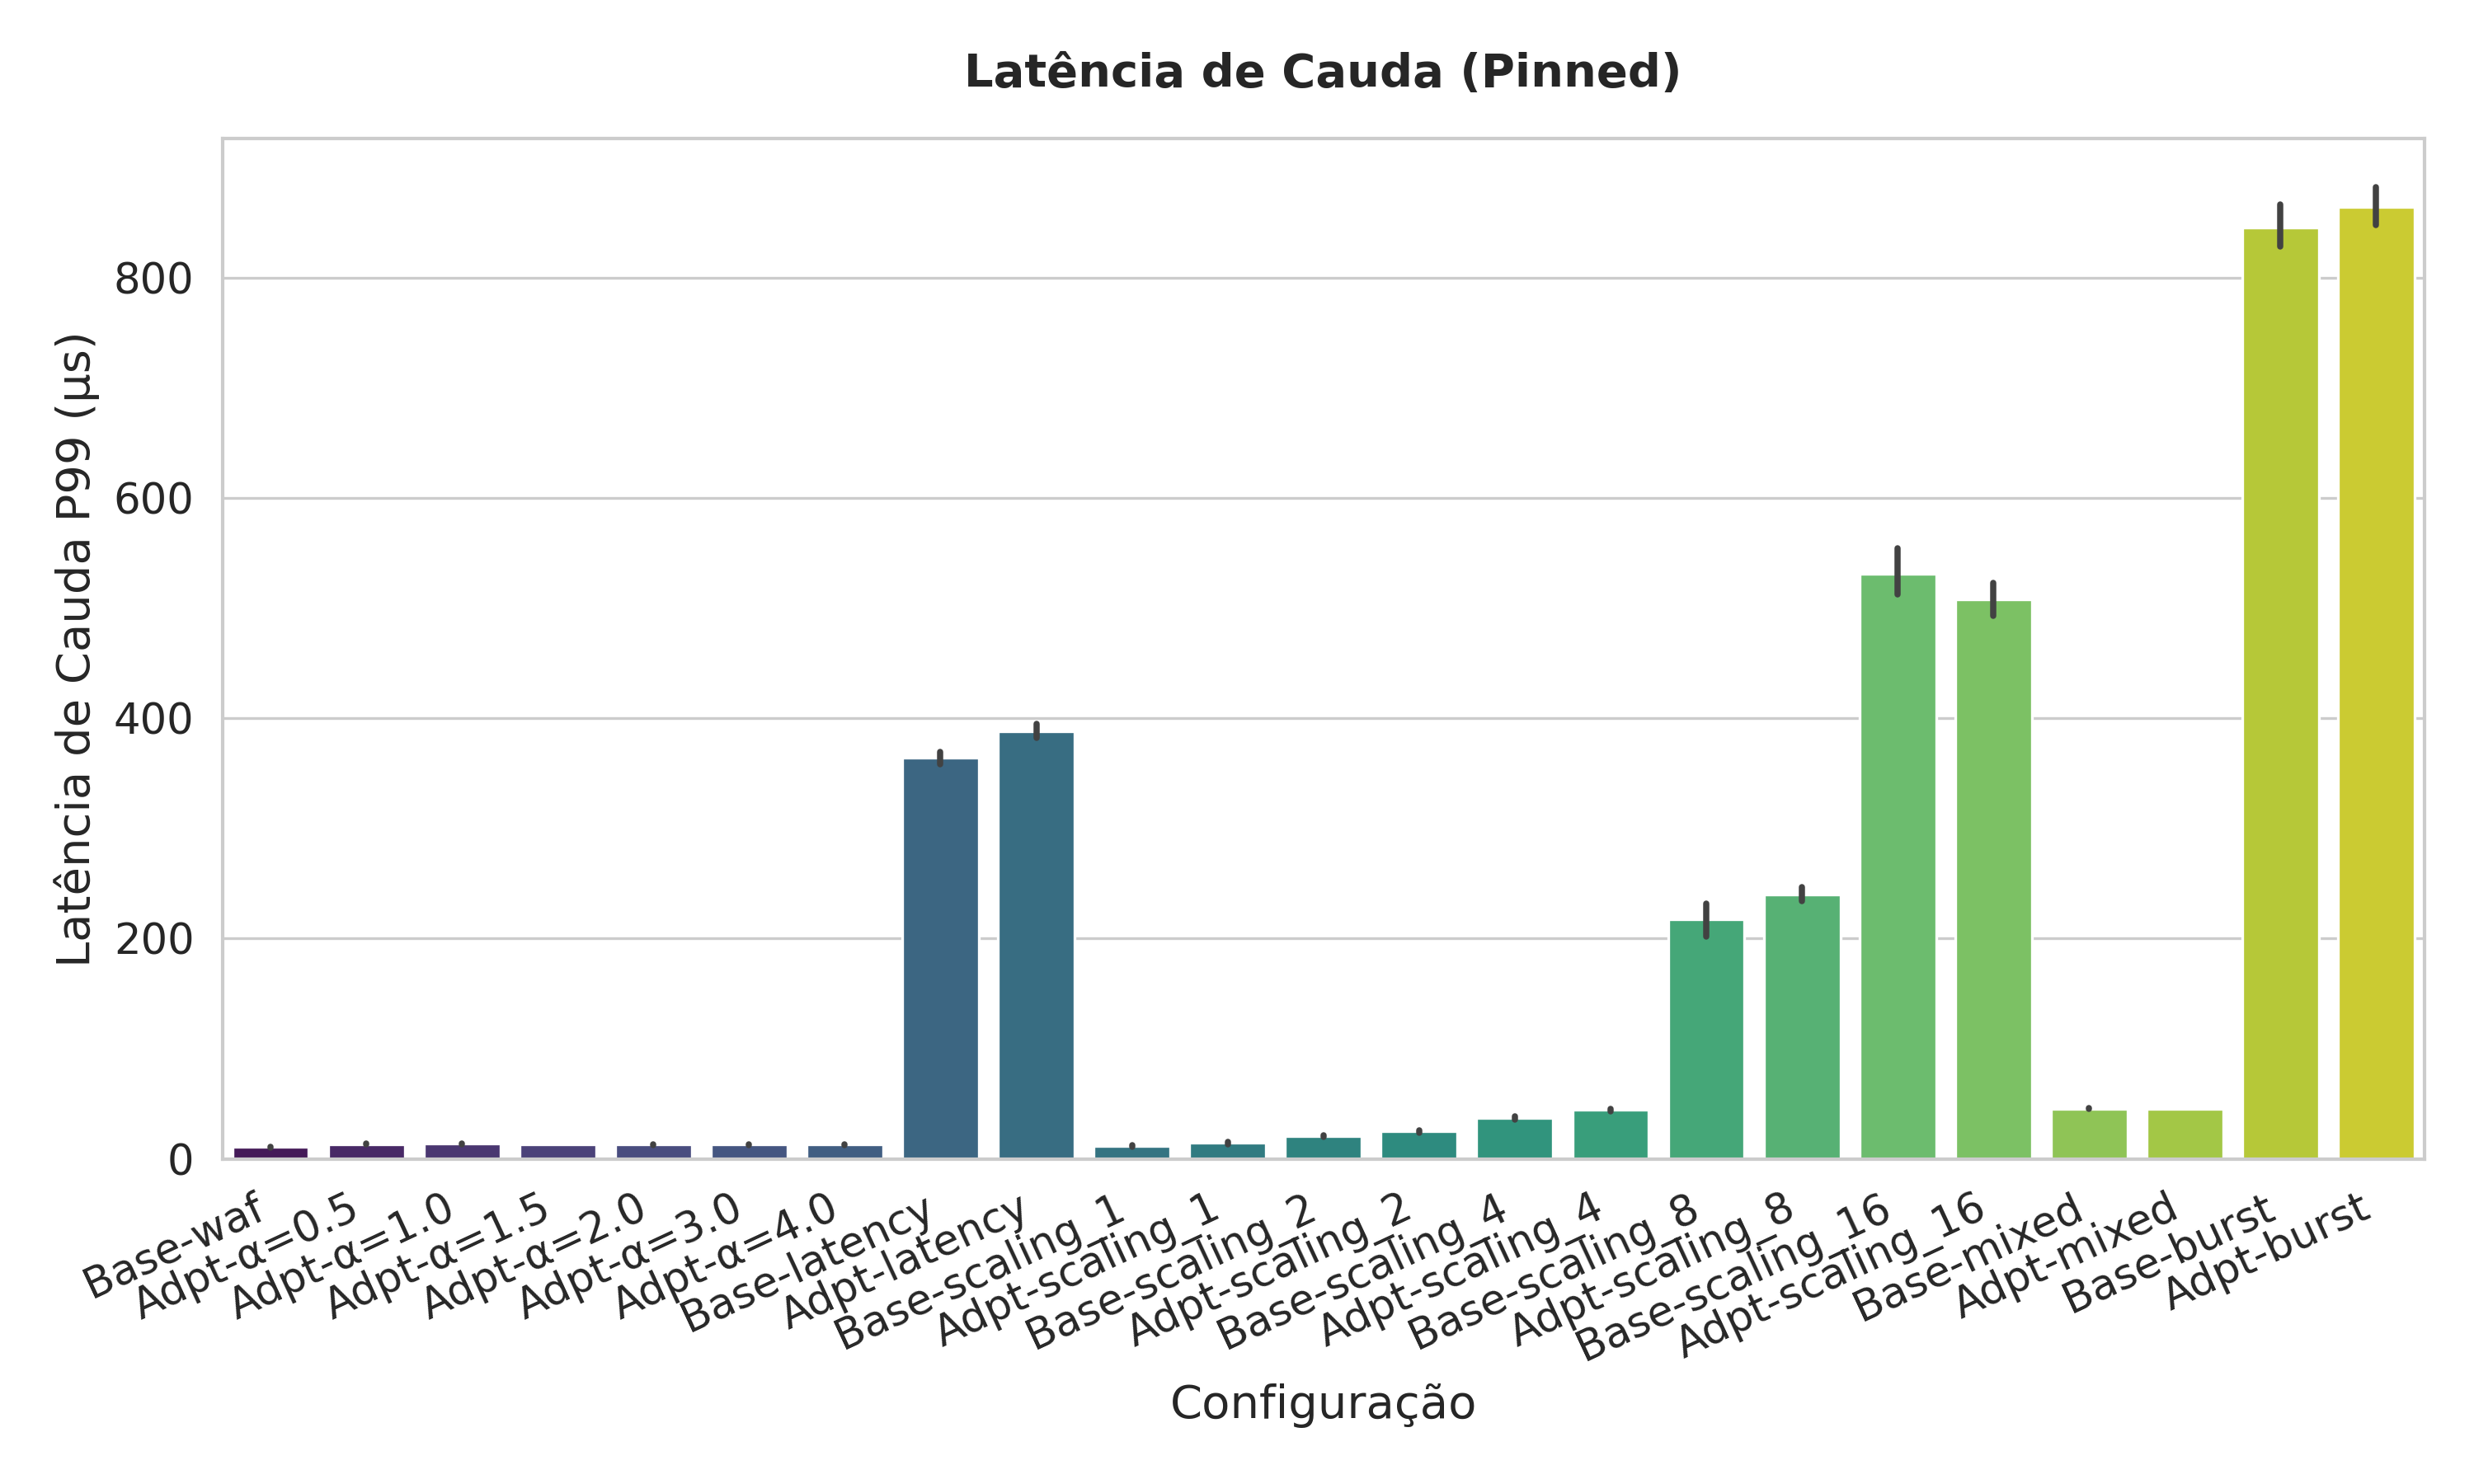
\includegraphics[scale=0.5]{figs/graphs/pinned/latency_p99.png}
\caption{Latência da cauda P99 em diferentes configurações. Mostra as \enquote{paradas} experimentadas pelos usuários durante a compactação.}
\label{fig:latency_p99_pinned}
\end{figure}

\begin{table}[h]
\centering
\caption{Latência de Cauda P99 ($\mu s$) - Ambiente Pinned}
\label{tab:latency_p99}
\begin{tabular}{lcc}
\hline
\textbf{Configuração} & \textbf{Média ($\mu s$)} & \textbf{Desvio Padrão} \\ \hline
Base-scaling\_8 & 217,88 & 38,15 \\
Adpt-scaling\_8 & 240,28 & 17,58 \\
Base-scaling\_16 & 531,03 & 54,17 \\
Adpt-scaling\_16 & 507,64 & 38,94 \\
Base-latency & 364,28 & 14,61 \\
Adpt-latency & 388,31 & 17,55 \\ \hline
\end{tabular}
\end{table}

A intervenção do nosso escalonador mostra seu brilho na contenção de degradações sob estresse massivo extremo. No teste com 16 \textit{threads} concorrentes (\textit{scaling\_16}), a mecânica de agendamento ingênua do sistema estático alcançou um engasgo perigoso, elevando o percentil P99 para 531,03 $\mu s$. A aplicação do algoritmo adaptativo reduziu com consistência essa latência para 507,64 $\mu s$, e mais importante, diminuiu agressivamente a volatilidade e o desvio padrão da latência (de $\pm 54,17 \mu s$ para $\pm 38,94 \mu s$). Isso certifica que o sistema consegue \enquote{adiar} ou gerenciar a prioridade do I/O, garantindo uma previsibilidade temporal muito maior para clientes externos.

\section{Eficiência das Compactações e Custo Computacional}

Um questionamento vital decorre das otimizações de latência: estaríamos diminuindo o trabalho de fundo (criando lixo excessivo) para melhorar o tempo de resposta superficial? A análise conjunta dos gráficos \ref{fig:compactio_cpu_pinned_a}, \ref{fig:compaction_count_pinned_b}, \ref{fig:compaction_ratio_c}  contrapõe essa preocupação com base em fatos quantitativos. 

\begin{figure}[h]
\centering
\subfloat[Tempo total de CPU gasto na compactação. Valores mais baixos sugerem um agendamento mais eficiente.\label{fig:compactio_cpu_pinned_a}]{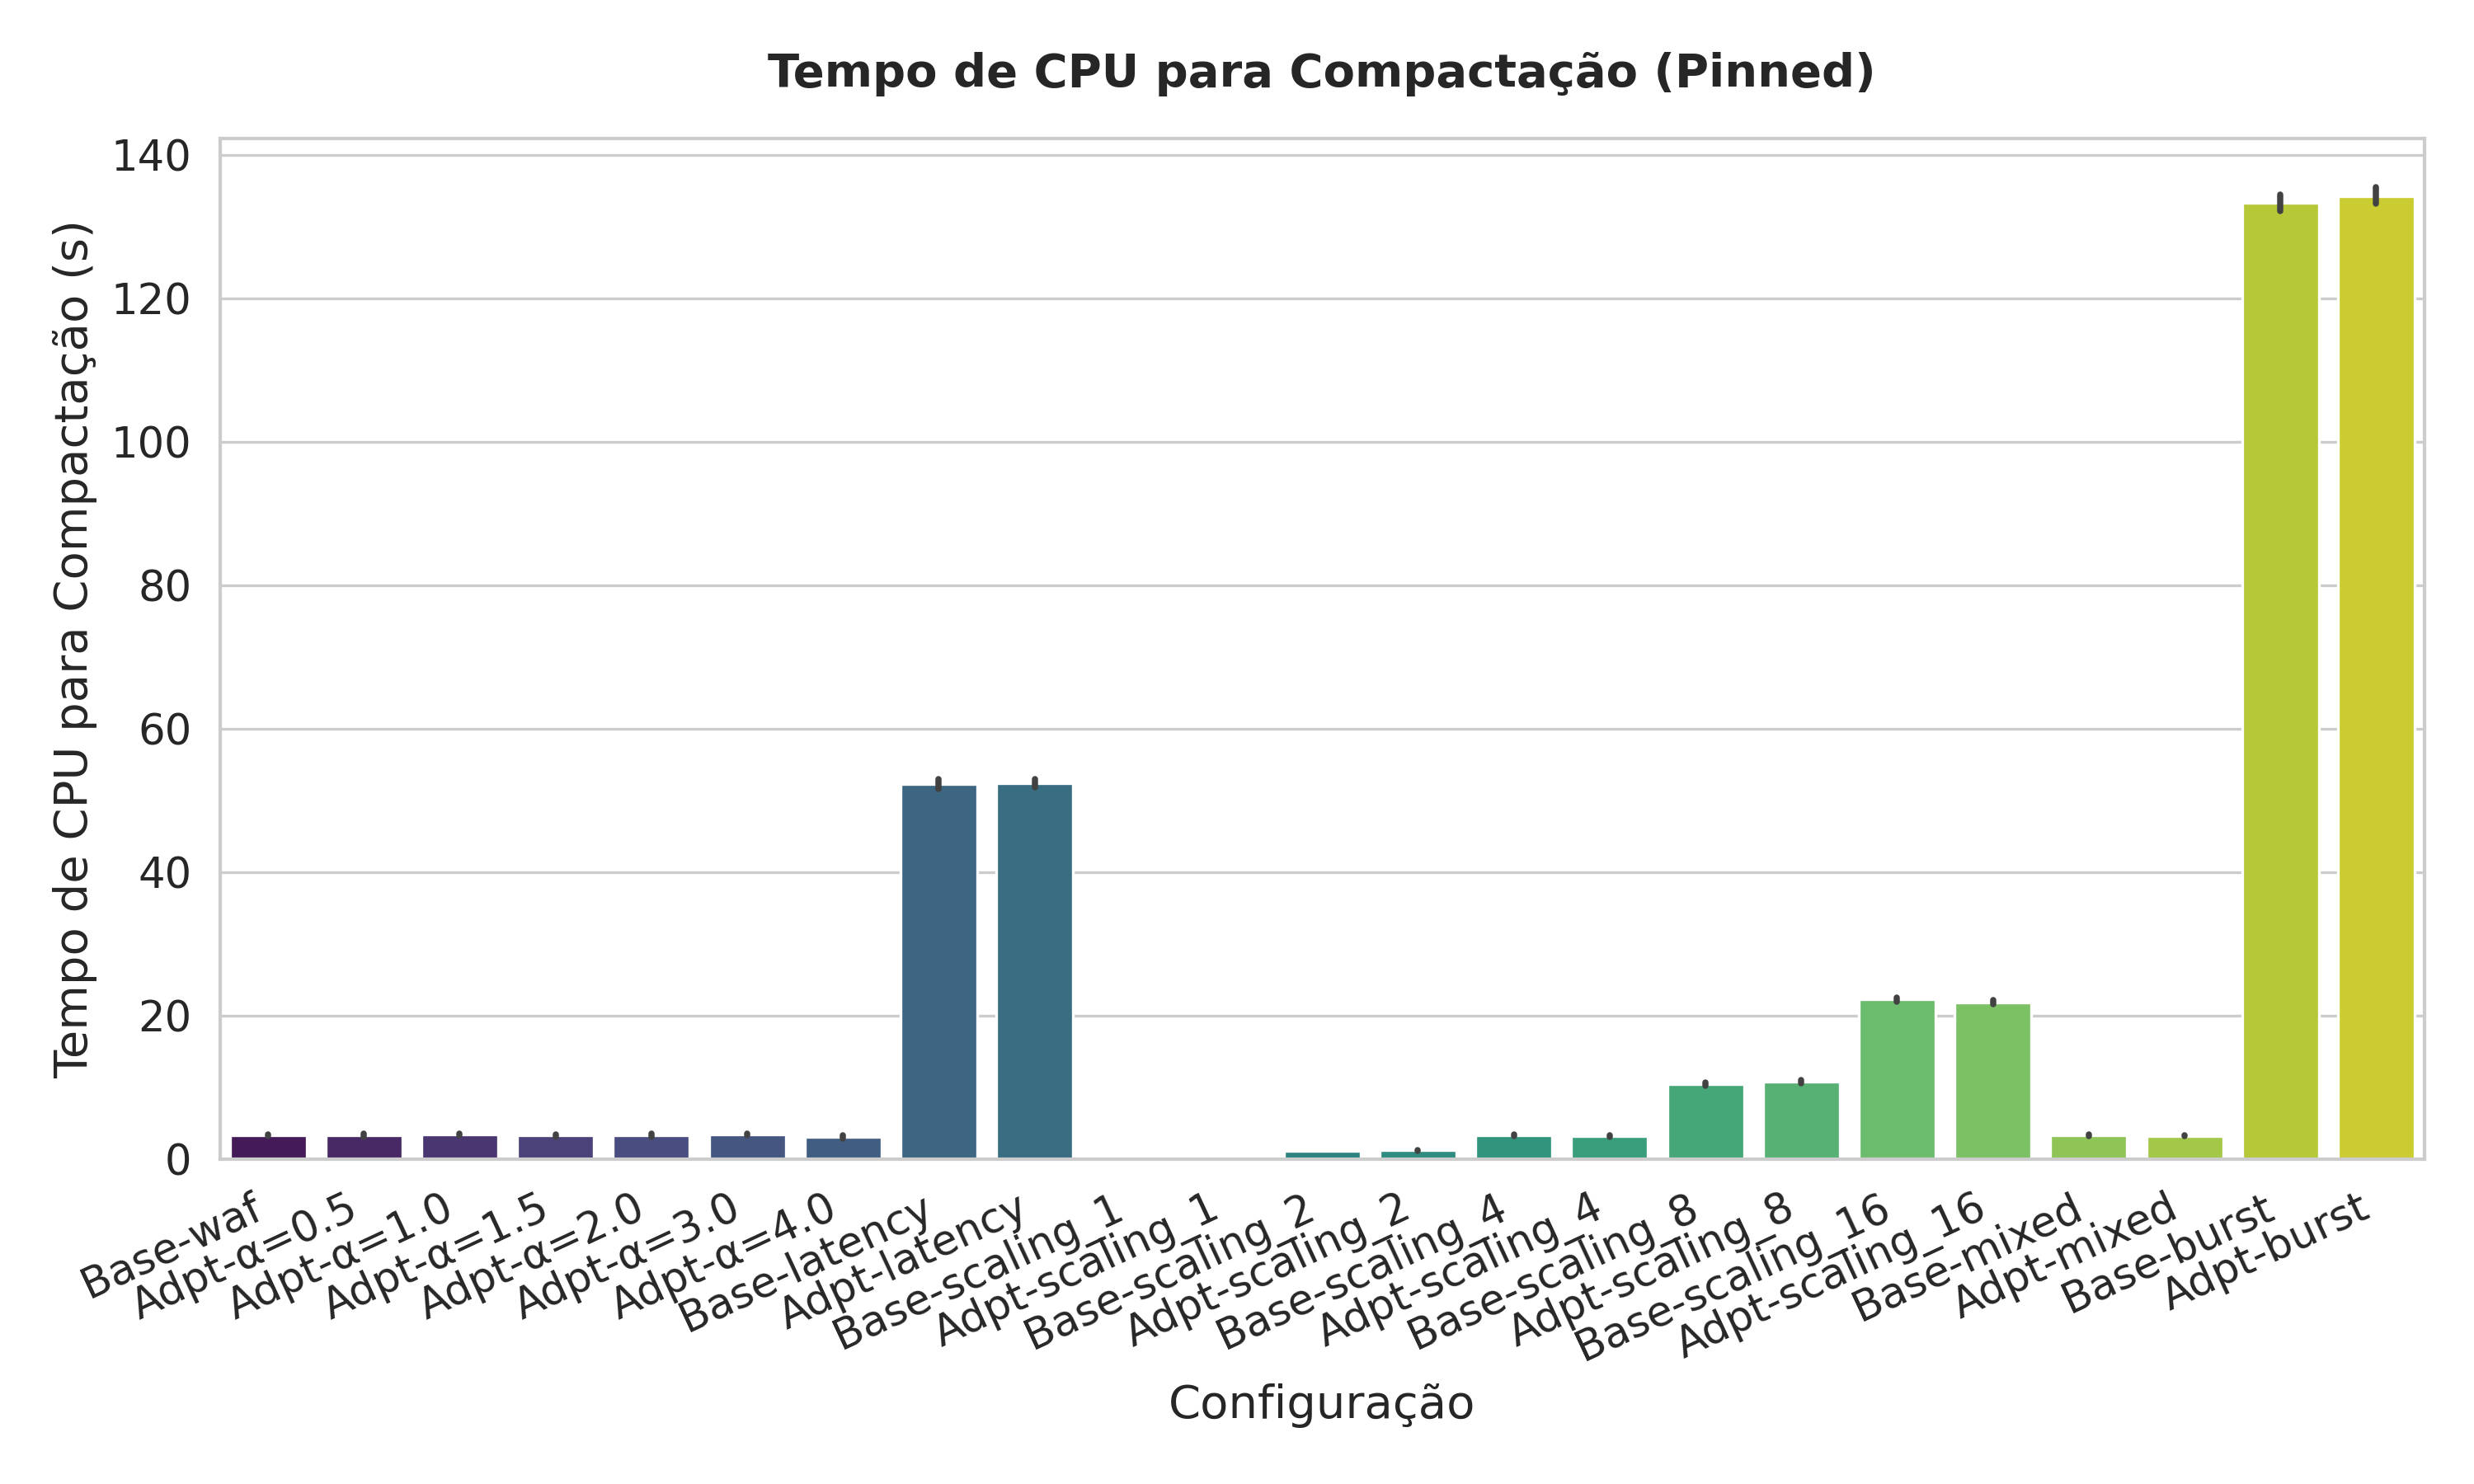
\includegraphics[width=0.6\textwidth]{figs/graphs/pinned/compaction_cpu.png}}\hfill
\subfloat[Número total de compactações realizadas.\label{fig:compaction_count_pinned_b}] {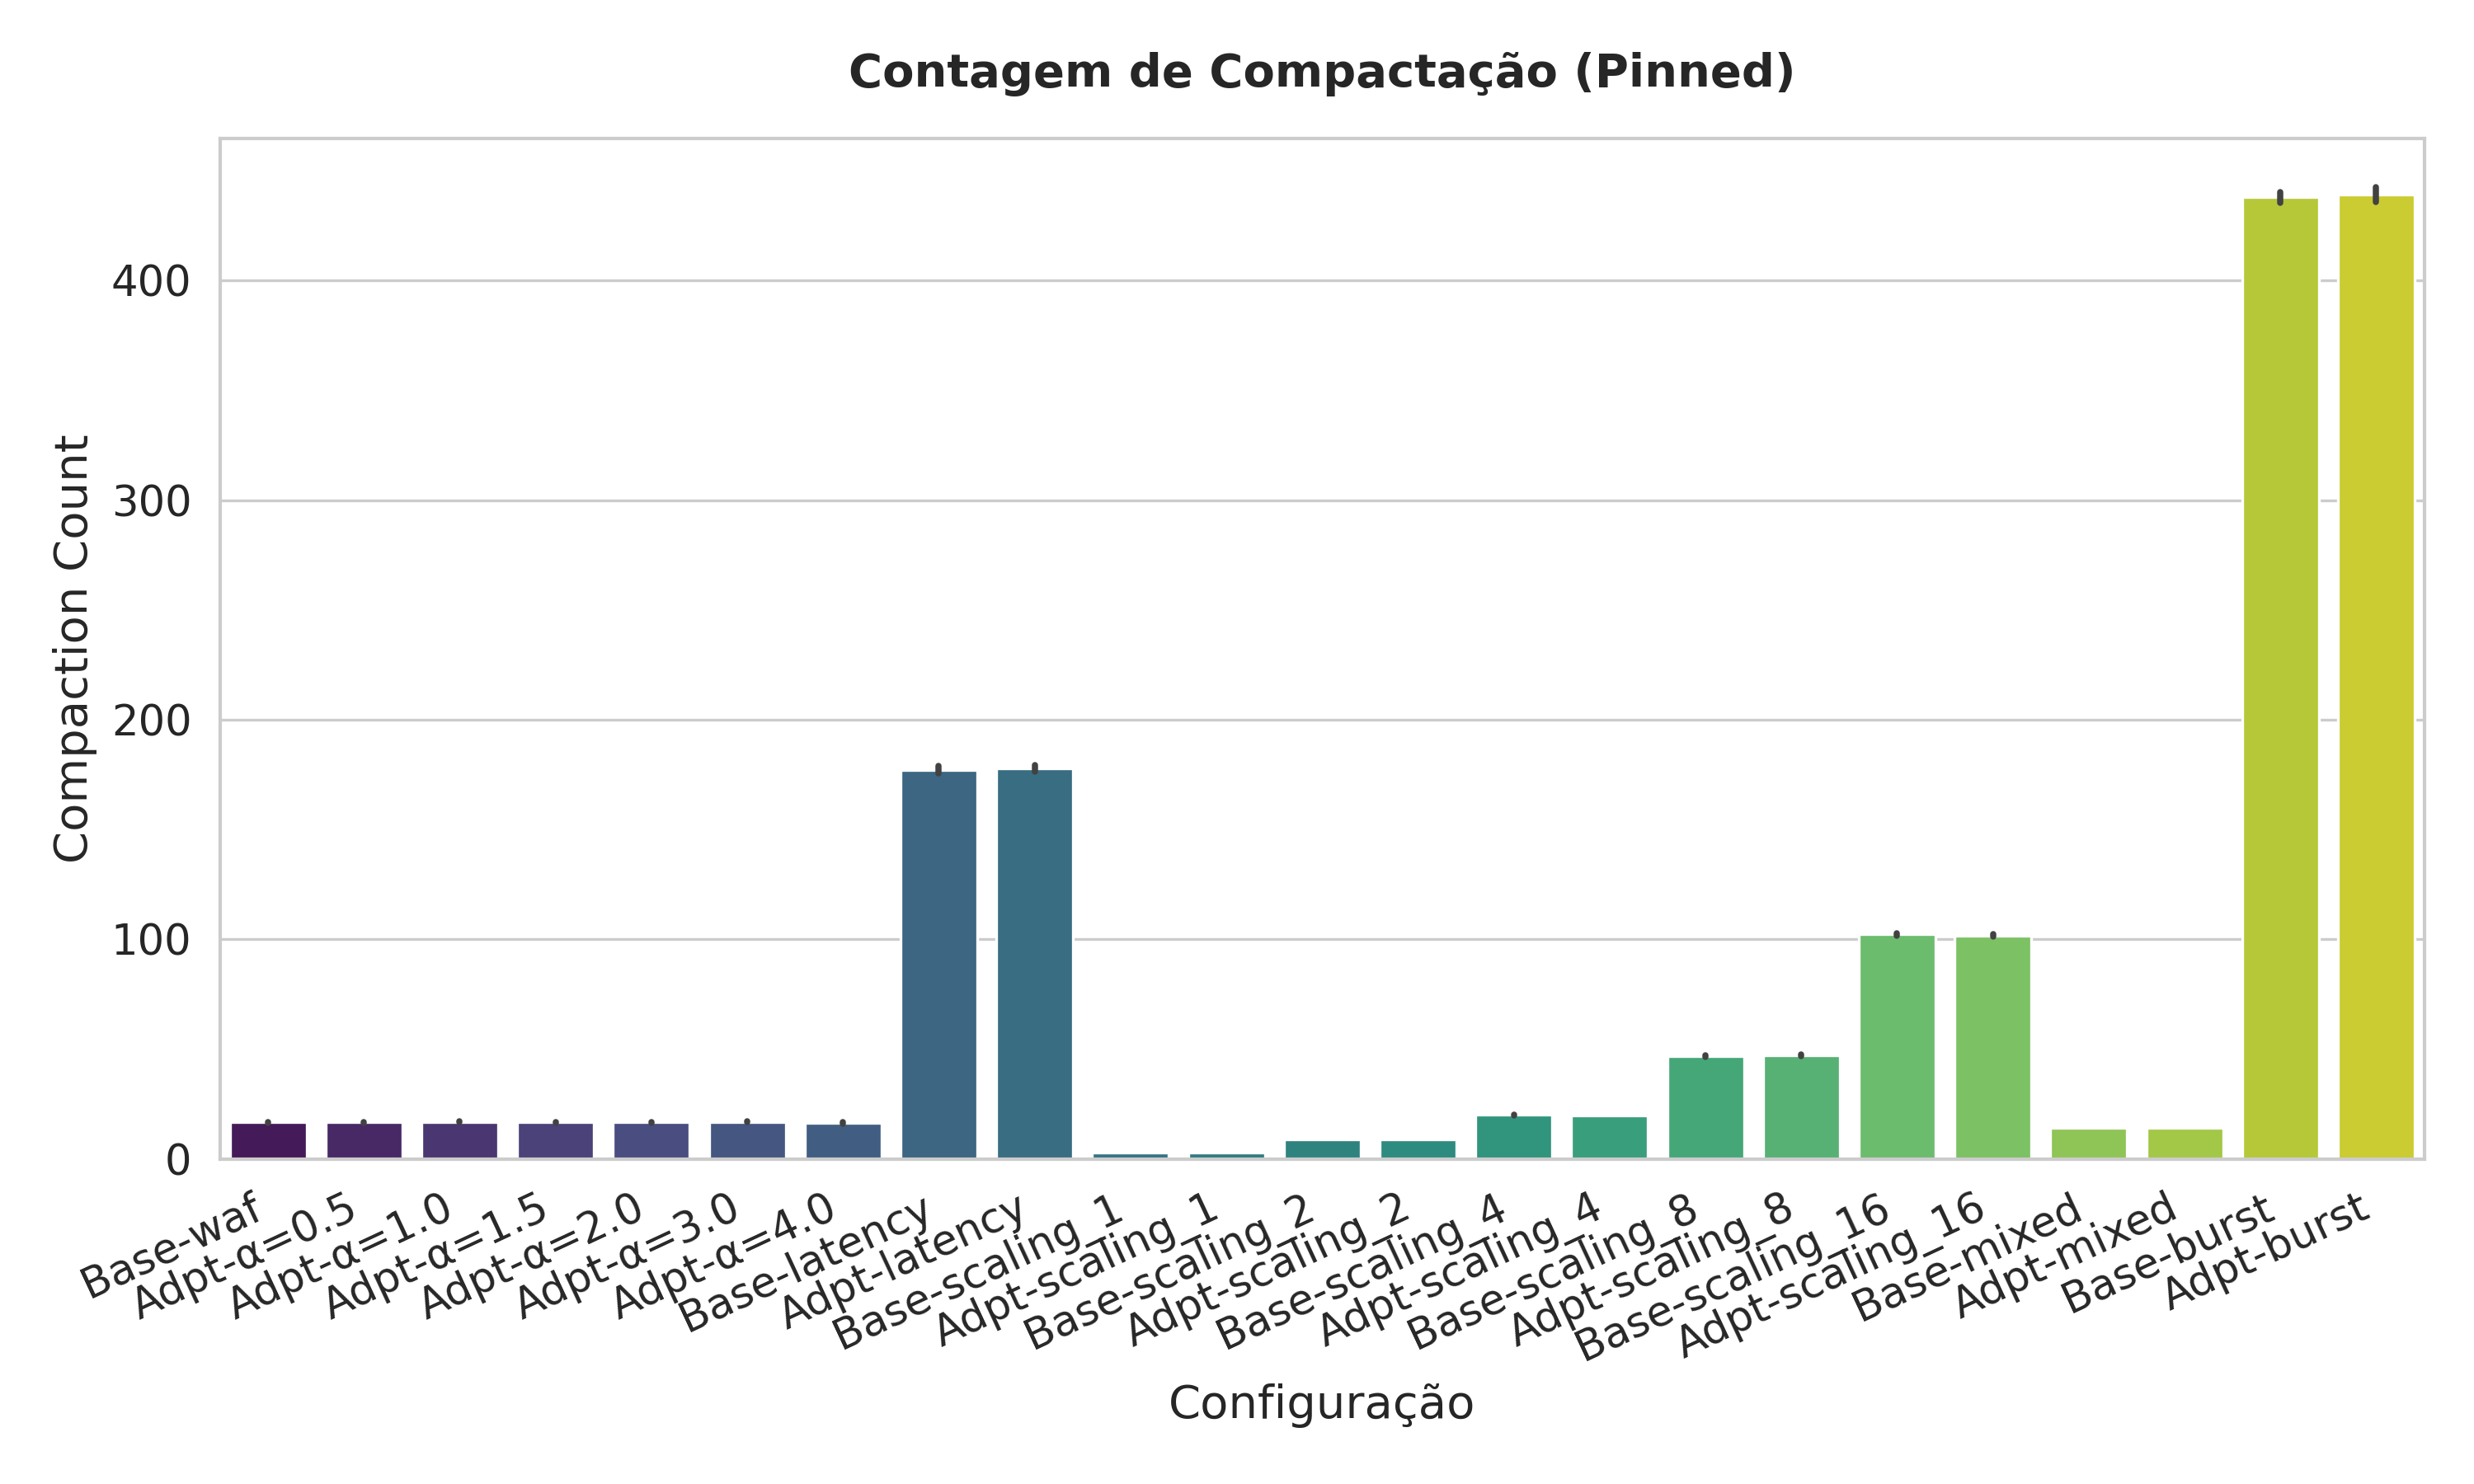
\includegraphics[width=0.6\textwidth]{figs/graphs/pinned/compaction_count.png}}\hfill
\subfloat[Fração do tempo total de execução gasto em compactação.\label{fig:compaction_ratio_c}]{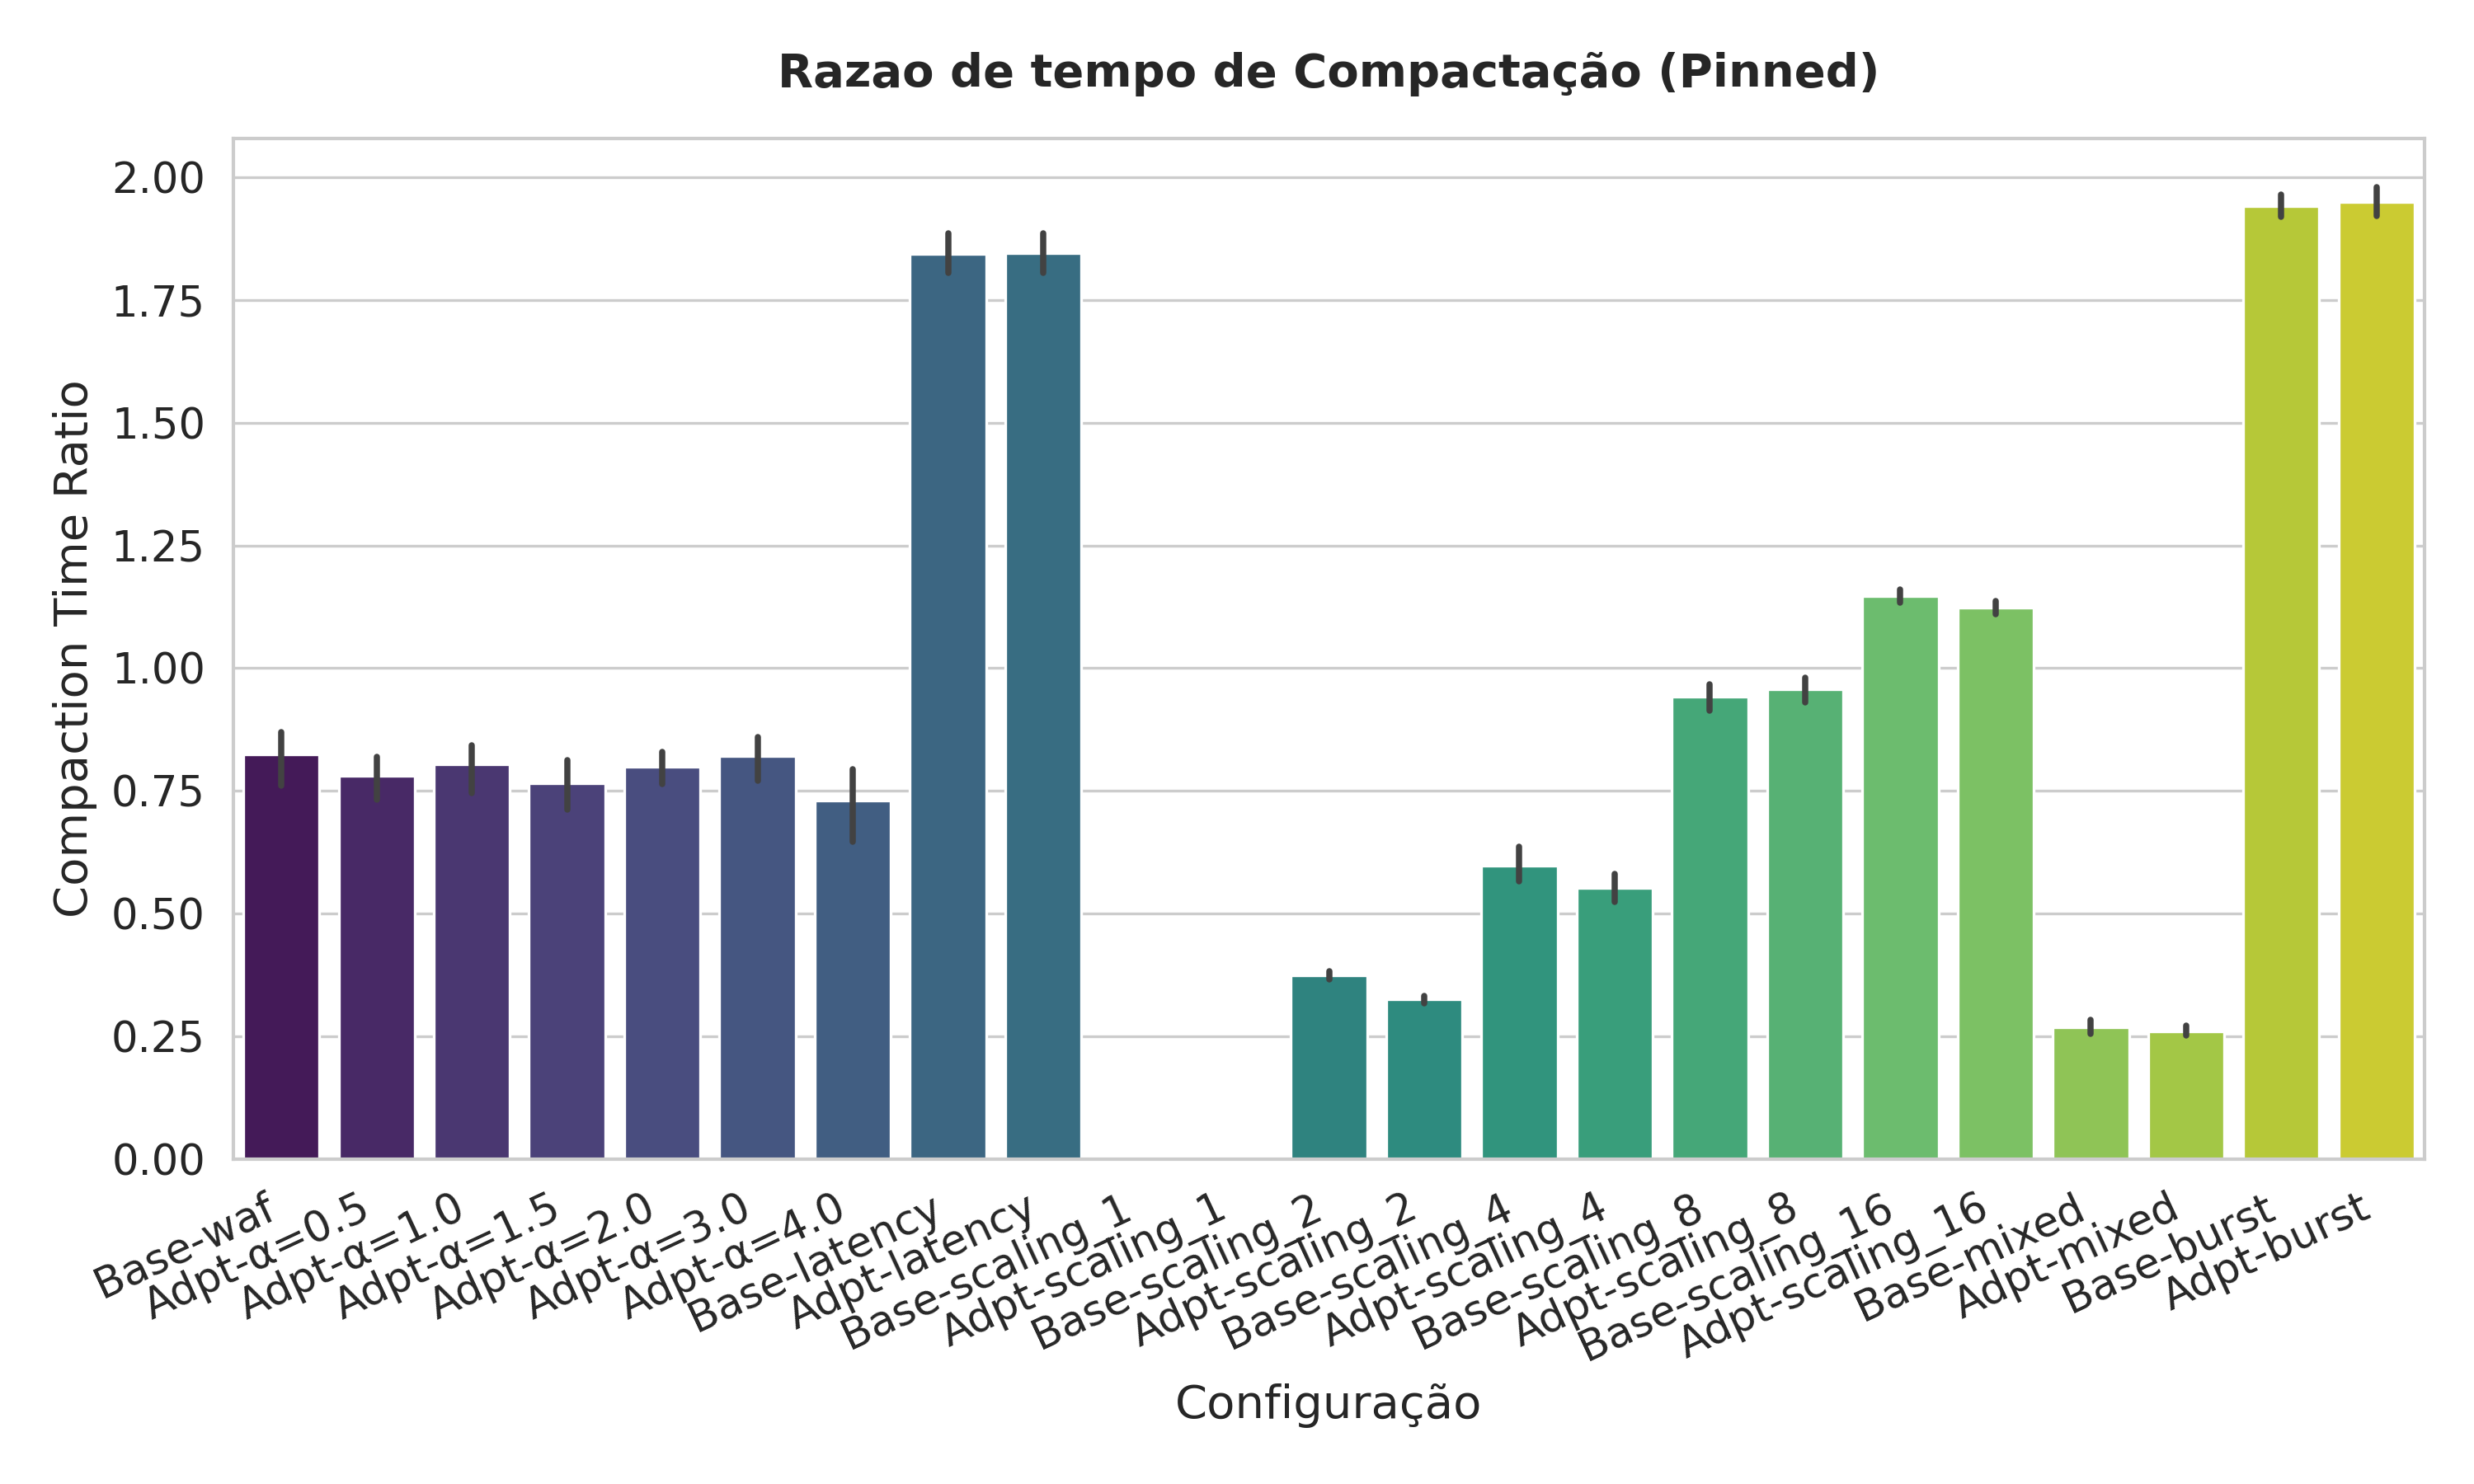
\includegraphics[width=0.6\textwidth]{figs/graphs/pinned/compaction_ratio.png}}
\caption{Gráficos sobre compactação} \label{fig:compaction_graphs}
\end{figure}

\begin{table}[h]
\centering
\caption{Métricas de Esforço de Compactação (Ambiente Pinned)}
\label{tab:compaction_effort}
\begin{tabular}{l|cc|cc}
\hline
\textbf{Configuração} & \textbf{Contagem (Total)} & \textbf{Desvio} & \textbf{CPU Gasto (seg)} & \textbf{Desvio} \\ \hline
Base-burst & 437,84 & 6,34 & 133,37 & 2,96 \\
Adpt-burst & 439,04 & 8,47 & 134,29 & 2,98 \\
Base-latency & 177,24 & 4,78 & 52,28 & 1,79 \\
Adpt-latency & 177,76 & 4,30 & 52,40 & 1,43 \\
Base-mixed & 14,12 & 0,33 & 3,29 & 0,26 \\
Adpt-mixed & 14,08 & 0,27 & 3,23 & 0,20 \\ \hline
\end{tabular}
\end{table}

Conforme a tabela \ref{tab:compaction_effort}, os volumes absolutos de trabalho executado pelo mecanismo original e pelo proposto são intrinsecamente idênticos. Durante as volumosas rajadas da carga (\textit{Burst}), o modelo padrão realizou em média $\sim$437 compactações custando 133,37 segundos de CPU; de forma análoga, nosso protótipo realizou $\sim$439 compactações consumindo 134,29 segundos. 

O cerne do escalonador implementada é explicitado aqui: o escalonador adaptativo entrega latências de P99 menores e sustenta a vazão \textbf{não porque abdica do trabalho}, mas porque utiliza o sensoriamento de I/O para agendar e distribuir esse montante exato de carga nos intervalos menos prejudiciais aos processos de \textit{frontend}. Trata-se de uma reorganização temporal eficiente, isenta de acúmulo patológico de registros inativos na PMEM.


\section{Durabilidade do Dispositivo e Amplificação de Escrita (WAF)}
Diferentemente das memórias voláteis tradicionais (DRAM), a tecnologia de Memória Persistente baseada na fase sólida de materiais apresenta limites operacionais no que tange a ciclos de gravação. O Fator de Amplificação de Escrita (WAF) afere quantas gravações físicas são necessárias por operação lógica de usuário, conforme retratado no gráfico \ref{fig:waf_pinned} e na tabela \ref{tab:waf_pinned}.

\begin{figure}[h]
\centering
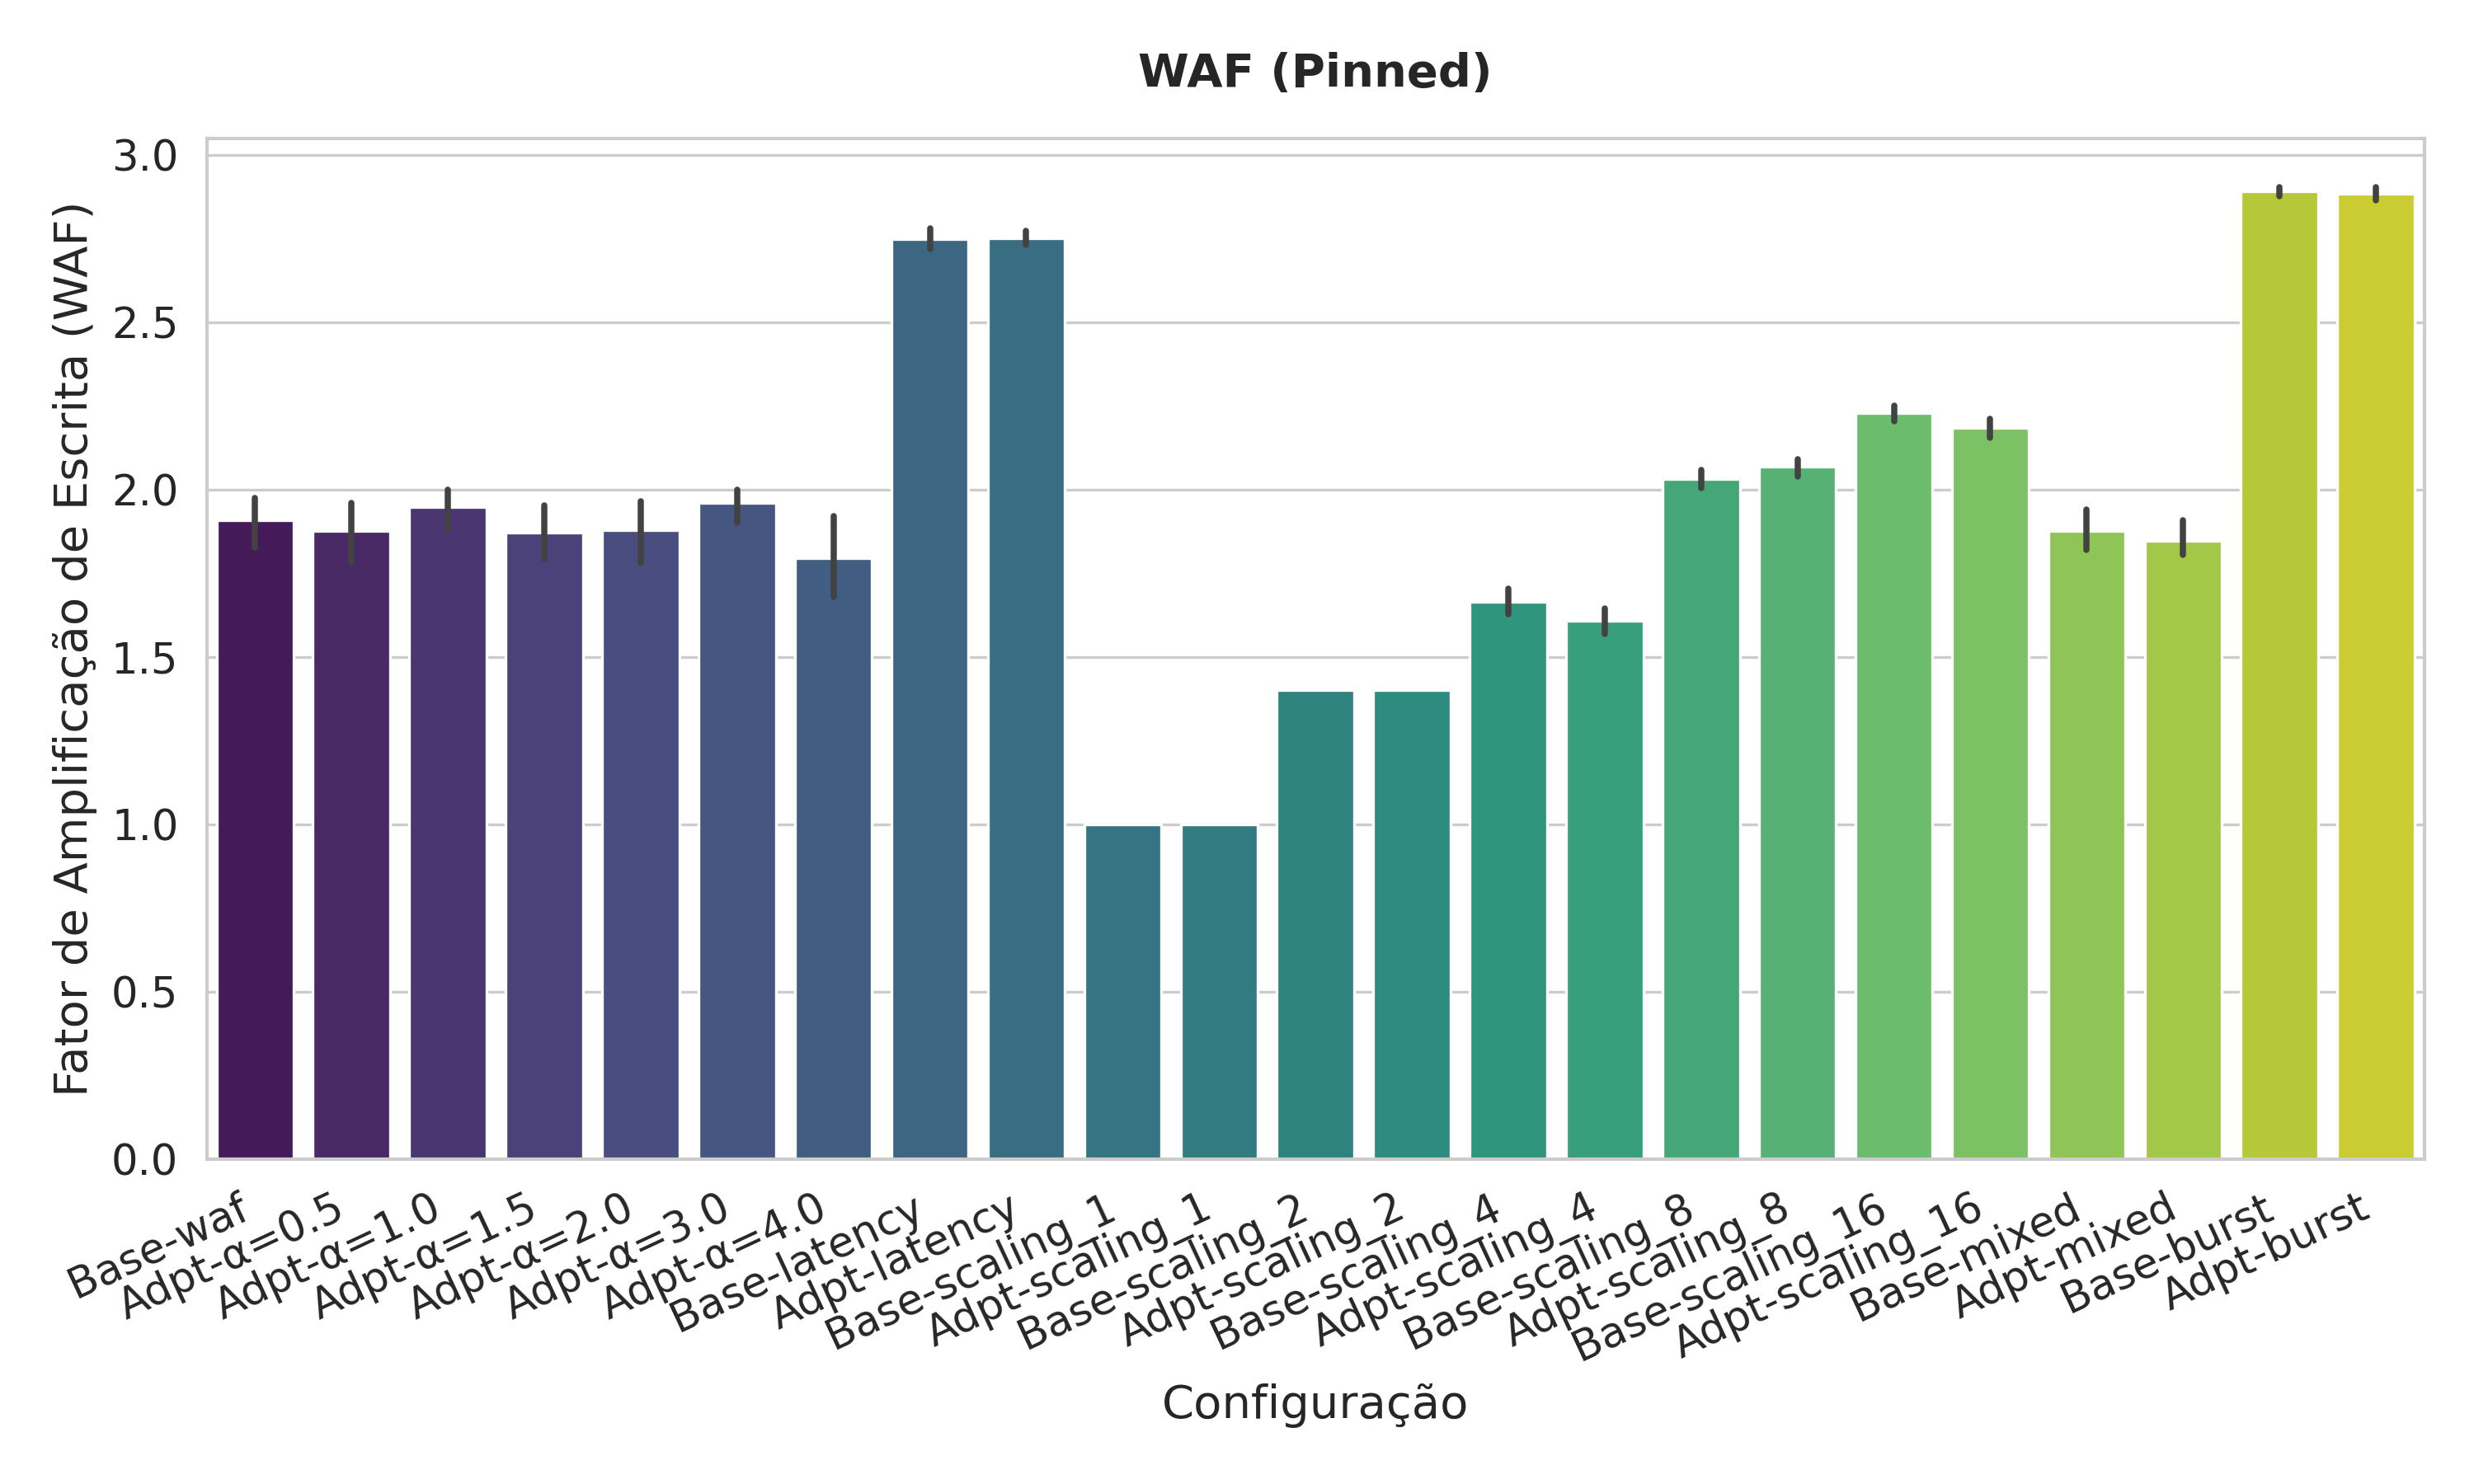
\includegraphics[scale=0.5]{figs/graphs/pinned/waf.png}
\caption{Vazão geral (operações por segundo) em todas as configurações. Quanto maior, melhor.}
\label{fig:waf_pinned}
\end{figure}

\begin{table}[h]
\centering
\caption{Métricas de Amplificação de Escrita - WAF (Ambiente Pinned)}
\label{tab:waf_pinned}
\begin{tabular}{lcc}
\hline
\textbf{Configuração} & \textbf{Média (WAF)} & \textbf{Desvio Padrão} \\ \hline
Base-burst & 2,8920 & 0,0400 \\
Adpt-burst & 2,8840 & 0,0554 \\
Base-latency & 2,7480 & 0,0770 \\
Adpt-latency & 2,7520 & 0,0510 \\
Base-mixed & 1,8760 & 0,1640 \\
Adpt-mixed & 1,8480 & 0,1388 \\
Base-scaling\_16 & 2,2280 & 0,0614 \\
Adpt-scaling\_16 & 2,1840 & 0,0688 \\ \hline
\end{tabular}
\end{table}

A amplificação manteve níveis altamente controlados, independentemente do tipo de sobrecarga aplicada. Destaca-se a eficiência na execução em cenário misto, apresentando WAF estável na casa de 1,84, com leve oscilação perante o motor base, bem como na contenção de carga pesada (\textit{scaling\_16}), alcançando WAF de 2,18. Isso responde definitivamente à viabilidade de adoção corporativa do projeto: a preservação do estado de saúde da mídia física não foi negligenciada em prol das métricas sistêmicas superficiais. O banco de dados operou em estado de otimização, estendendo a vida útil do \textit{hardware} adjacente sem incorrer em penalizações transacionais.

\section{Ameaças à Validade}

Nesta seção, discutem-se as limitações e os fatores que podem influenciar a interpretação dos resultados, garantindo a transparência necessária para a validação científica do Escalonador Adaptativo proposto.

\subsection{Validade Interna}
A validade interna refere-se à confiança de que as melhorias observadas (como a redução do P99 no cenário \textit{scaling\_16}) foram causadas pelo algoritmo adaptativo e não por ruídos externos. 

Uma ameaça relevante é a interação entre o nosso escalonador e as políticas nativas de \textit{write stall} do RocksDB. Embora tenhamos isolado o comportamento do agendamento de compactação, o motor original possui mecanismos de defesa que podem desacelerar a escrita do usuário se os níveis da árvore LSM acumularem excessivamente. Outro fator de interferência é o escalonador do \textit{kernel} Linux; mesmo no cenário \textit{Pinned}, interrupções de hardware e processos do sistema operando nos mesmos núcleos podem inserir variações na latência, o que explica os desvios-padrão observados de até $\pm 54,17 \mu s$ em cargas intensas.

\subsection{Validade Externa}
A validade externa diz respeito à generalização dos resultados. Nossos testes foram conduzidos em um ambiente de hardware específico e de alto desempenho: processador Intel Xeon Gold 5317 e Memória Persistente Intel Optane. 

É possível que os ganhos de desempenho e a redução de WAF não se comportem da mesma forma em mídias de armazenamento mais lentas, como SSDs SATA ou HDDs convencionais, onde a latência de I/O é ordens de grandeza superior à da PMEM. Além disso, embora os \textit{workloads} (\textit{Mixed, Burst, Scaling, Latency}) tenham sido desenhados para cobrir os principais padrões de acesso do \texttt{db\_bench}, eles permanecem sendo cargas sintéticas. Aplicações reais com acessos altamente assimétricos ou padrões de dados comprimíveis podem apresentar resultados distintos.

\subsection{Validade de Construção}
Esta categoria avalia se as métricas escolhidas realmente representam o que pretendemos medir. Utilizamos o Fator de Amplificação de Escrita (WAF) como métrica primária para durabilidade da Memória Persistente. No entanto, o desgaste físico real das células de NVM depende também da localidade das escritas e do alinhamento de blocos, detalhes que o WAF, sendo uma razão lógica, simplifica. Da mesma forma, o uso do percentil P99 é um excelente indicador de SLA, mas pode não capturar anomalias extremas que seriam visíveis apenas em percentis superiores, como P99.9 ou P99.99.

\subsection{Validade de Conclusão}
A validade de conclusão trata da robustez estatística. Para mitigar esta ameaça, adotamos um rigoroso protocolo de 25 repetições para cada teste, permitindo o cálculo de médias e desvios-padrão estáveis. 

Contudo, uma limitação admitida é a ausência de testes de hipótese formais (como o teste t de Student ou ANOVA) para confirmar a significância estatística de todas as variações. Embora as tendências nos gráficos de vazão (\textit{throughput}) e latência pareçam claras, a sobreposição de intervalos de desvio em certos cenários de baixa carga sugere que, para esses casos específicos, a distinção entre o modelo \textit{Base} e o \textit{Adaptativo} pode ser influenciada pela variância inerente ao sistema operacional.

\subsection{Síntese das Limitações}
Em resumo, os resultados apresentados devem ser interpretados sob as seguintes premissas:
\begin{itemize}
    \item Os benefícios de desempenho são maximizados em ambientes com afinidade NUMA e uso de Memória Persistente;
    \item O sistema assume que a carga de trabalho futura guarda correlação com a telemetria coletada no passado imediato;
    \item As conclusões baseiam-se em médias estatísticas de 25 execuções, refletindo o comportamento esperado sob condições controladas de laboratório.
\end{itemize}